\documentclass[conference,letterpaper]{IEEEtran}
\IEEEoverridecommandlockouts
% The preceding line is only needed to identify funding in the first footnote. If that is unneeded, please comment it out.

\usepackage{cite}
\usepackage{natbib}
\usepackage{amsmath,amssymb,amsfonts}
\usepackage{algorithmic}
\usepackage{graphicx}
\usepackage{textcomp}
\usepackage{xcolor}
\usepackage{graphicx}
\usepackage{subfigure}               %²åÈë²¢ÅÅ͌Ƭ
\usepackage{CJK}                     %²åÈëÊýѧ¹«Êœ
\usepackage{indentfirst}             %²åÈëÊýѧ¹«Êœ
\usepackage{amsmath}                 %²åÈëÊýѧ¹«Êœ
\usepackage{upgreek}                 %Æœ·œÎ¢Ã×µ¥Î»
\usepackage{tabu}                    %²åÈë±ížñ
\usepackage{tabularx}
\usepackage{booktabs}
\usepackage{threeparttable}
\usepackage{multirow}
\usepackage{multicol}
\usepackage{arydshln}                %²åÈë±ížñ
\usepackage{makecell}                %ŒÓºÚijžùÏß
\usepackage{amsmath}
\usepackage{geometry}
\usepackage{float}
\usepackage{caption}
\usepackage{amsmath}
\usepackage{tabularx}
\geometry{a4paper,left=2cm,right=2cm,top=2.5cm,bottom=4.6cm}
\renewcommand\refname{\textbf{\large REFERENCES}}
\setlength{\parindent}{0.63cm}
\setlength{\columnsep}{0.8cm}
\def\BibTeX{{\rm B\kern-.05em{\sc i\kern-.025em b}\kern-.08em
    T\kern-.1667em\lower.7ex\hbox{E}\kern-.125emX}}
\makeatletter
\renewcommand{\section}{\@startsection{section}{1}{0mm}
    {-\baselineskip}{0.001\baselineskip}{\bf\leftline}}
\makeatletter
\renewcommand{\subsection}{\@startsection{subsection}{1}{0mm}
	{-\baselineskip}{0.001\baselineskip}{\bf\leftline}}
\makeatletter
\captionsetup[figure]{labelfont=it,textfont={it},name=Figure}
\captionsetup[table]{name={TABLE},labelsep=period}
%\usepackage[labelfont=it,textfont=it]{caption}
\begin{document}
\title{ \Large\textbf{ Stochastic Circuit Design Based on Exact Synthesis}\vspace{-1.2em} }
%\thanks{The work was supported by NSFC under Grant 61871242.}
\author{\IEEEauthorblockN{\textit{\large Xiang He, and Zhufei Chu$^*$}}
\IEEEauthorblockA{\large EECS, Ningbo University, Ningbo 315211, China \\ $^*$ Email: chuzhufei@nbu.edu.cn \vspace{-0.5em}}}

\maketitle
\section*{\textbf{\large ABSTRACT}}
Stochastic computing enables computationally complex arithmetic using binary numbers converted to sto-chastic bitstreams. A large number of applications have used stochastic computing due to its fault-tolerant nature. However, stochastic circuit synthesis presents a larger solution space when compared to classical logic synthesis. Previous methods synthesize stochastic circuits using a heuristic method. In this paper, a novel exact synthesis method using Boolean satisfiability (SAT) is proposed to obtain an optimal stochastic circuit represented by majority-inverter graphs (MIGs). The experimental results suggest that the proposed approach can achieve 21\% area reduction, 4\% delay improvement, with a 3\% mean absolute error trade-off.    
\vspace{3ex}

%\begin{IEEEkeywords}
%stochastic computing; exact synthesis; logic synthesis; majority
%\end{IEEEkeywords}

\section*{\textbf{\large INTRODUCTION}}
Many constraints limit modern circuit development, such as voltage variations, thermal variations, and soft errors. These physical phenomena are susceptible to errors, thus reliability has become an important issue. Stochastic computing (SC) has received increasing attention as an unconventional computing method for solving these problems. SC is unique in that it represents and processes information in the probabilistic form and is highly fault-tolerant for bit flips. SC converts numbers $x\in[0,1]$ into stochastic bitstreams consisting of only 0 and 1. 
Each bit has a probability $x$ of being a one and probability $1-x$ of being a zero in the bitstream. The values are represented by the probability of the one in the bitstream. For example, (0,1,0,0) and (0,0,0,1) are potential representations of the value 0.25 as the digit `1' presents once in the bitstream with length four. Numbers are normally stored in long bitstreams where a few bits are flipped without a significant difference in value. By converting numbers into random bitstreams, SC %stochastic computing 
transforms a complex computing unit into a simple circuit with gates. Thus many arithmetic operations can be implemented with very simple logic circuits. For example, multiplication in SC %stochastic computing
 can be implemented with an AND gate if the two input stochastic bitstreams are independent, as shown in Figure~\ref{fig:sto}. 
SC has been applied to many applications~\cite{Promise-and-Challenge} as image processing, neural networks, decoding LDPC code, and filter design.
\vspace{3ex}


\begin{figure}[t]
	\centering
	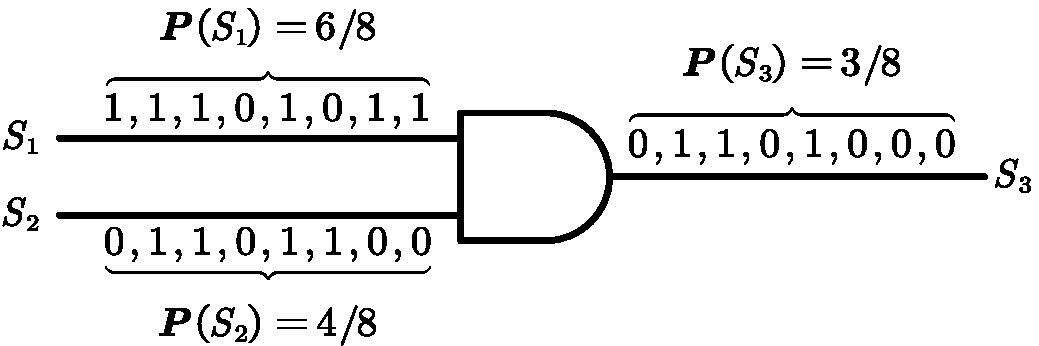
\includegraphics[width=3.5in]{fig/AND3.pdf}
	\caption{\label{fig:sto}AND gate performs multiplication by stochastic bitstreams.}  \vspace{-3.5ex}
\end{figure}

Multiple distinct Boolean functions can be used to compute the same function, which has a large solution space for the synthesize of stochastic circuits. 
Researchers have recently proposed several approaches for synthesizing functions in SC. 
A method that is currently being implemented~\cite{Cube-Assignment} is based on assigning cubes (i.e., product terms) to the on-set of the Boolean function. The heuristics, however, do not yield optimal solutions. Exact synthesis is a new approach to finding Boolean networks that represent Boolean functions and respect given constraints. Exact synthesis allows one to find optimum networks, e.g., in size or depth. In this paper, we employ an exact synthesis method to obtain an optimal SC circuit represented by MIGs. Experimental results have shown that the exact synthesis approach outperforms the heuristic approach in terms of area and delay.

\section*{\textbf{\large BACKGROUND}}
\subsection*{\textbf{Stochastic Computing Circuits }}
A general form of the stochastic circuit is shown in Figure~\ref{fig2}, which is a combinational circuit. For a function of single variable $x$, the stochastic number generator (SNG) generates $n$ independent inputs $X_{1}, \ldots, X_{n}$, whose probability is $x$, where $n$ is the highest degree of the variable $x$ in the function. SNGs typically consist of a pseudo-random number generator and a comparator. A linear feedback shift register (LFSR) generates $m$ inputs $Y_1, \ldots, Y_m$ with probability 0.5. The stochastic bitstreams of these $n+m$ inputs are processed by a combination logic circuit.

\begin{figure}[t]
	\centering
	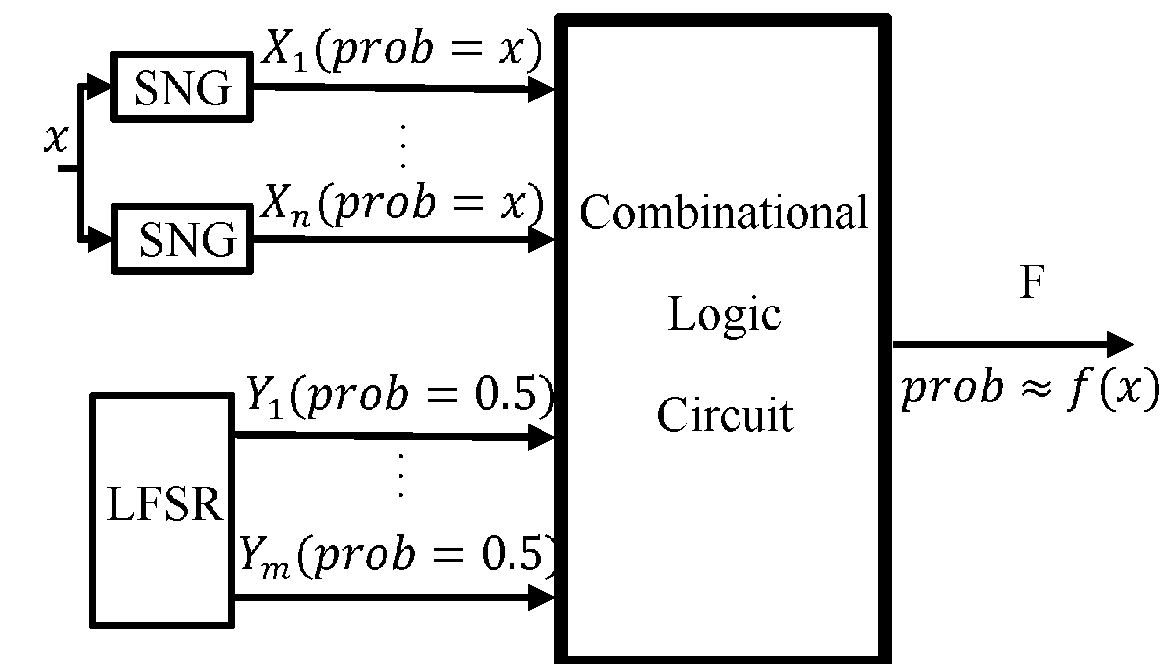
\includegraphics[width=3in]{fig/sc.pdf}	
	\caption{\label{fig2}A general form of stochastic computing circuits.} \vspace{-2ex}
\end{figure}

For $i\in[0,n]$, let $G(i)$ represents the number of minterms $(X_{1}, \ldots, X_{n}, Y_{1}, \ldots, Y_{m})$ that satisfying $F(X_{1}, \ldots, X_{n}, Y_{1}, \ldots, Y_{m})=1$ and $\sum_{j=1}^{n} X_{j}=i$. $(G(0), \ldots, G(n))$ is recorded as the \emph{problem vector}~\cite{Cube-Assignment}. For example, $(0, 3, 2)$ is a problem vector using the Karnaugh map shown in Table~\ref{tab:tt} with $n=2$ and $m=2$. Its output probability realizes the function
\begin{equation}
f(x)=\frac{3}{4} x(1-x)+\frac{2}{4} x^{2}.\vspace{-2ex}
\end{equation}


\begin{table}[htbp]
\setlength{\abovecaptionskip}{0.cm}
\setlength{\belowcaptionskip}{0.pt}
\setlength{\tabcolsep}{1mm}
\caption{The Karnaugh map of a Boolean function with problem vector $(0, 3, 2)$.}
\centering \label{tab:tt}
\begin{tabular}{p{2cm}<{\centering} p{1.25cm}<{\centering} p{1.25cm}<{\centering} p{1.25cm}<{\centering} p{1.25cm}<{\centering}}
%\begin{tabularx}{\linewidth}{lXXXX}
\toprule
$\mathrm{Y}_{1} \mathrm{Y}_{2} \backslash \mathrm{X}_{1} \mathrm{X}_{2}$ & 00 & 01 & 11 & 10 \\
\midrule
00 &0 & 1 & 1 & 1 \\
01 &0 & 1 & 1 &0 \\
11 &0 &0  &0  &0 \\
10 &0 &0 &0   &0 \\
\bottomrule
\end{tabular}
\end{table}

The Boolean function shown in Table~\ref{tab:tt} is represented in a simplified sum-of-product (SOP) form
\begin{equation}
F=X_{2}\bar{Y_{1}}+X_{1} \bar{Y_{1}}\bar{Y_{2}}.
\end{equation}

Consequently, a problem vector can be used as a logical circuit for stochastic computation, but there are many kinds of Boolean functions for implementing the same problem vector.
The problem vector $(0, 3, 2)$ indicates that $G(0)=0$, $G(1)=3$, and $G(2)=2$.
As shown in Table~\ref{tab:tt}, column ``00'' represents $G(0)$. Since $G(0)=0$, then all the entries under this column must be all zero.
Similarly, the column ``11'' represents $G(2)$, then we should assign two (i.e. $G(2)=2$) `1's into 4 entries. Thus, there are $\binom{4}{2}=6$ potential assignments.
Furthermore, the columns ``01'' and ``10'' represent $G(1)$, we should assign three `1's into 8 entries, which results in $\binom{8}{3}=56$ possibilities.
Therefore, Table~\ref{tab:tt} demonstrates just one of the $\binom{4}{2} \times \binom{8}{3} = 336$ Boolean functions of the problem vector $(0, 3, 2)$.

\subsection*{\textbf{SAT-based Exact Synthesis}}
Exact synthesis is the problem of finding optimal logic networks by giving a set of primitives.
Knuth proposed a SAT-based method for optimum Boolean evaluation~\cite{knuth}. 
The aim is to answer whether if there exists an $r$-step normal Boolean chain that computes $a$ given functions $g_1$, $\ldots$, $g_a$ on $b$ variables. The concept of Boolean chain is a directed acyclic graph (DAG) in which every vertex corresponds to a $k$-input Boolean operator. 
Given defined Boolean variables, SAT clauses are constructed to constraint correct Boolean operations and connections.
A brief introduction is shown as the following. 

1) Variables: For $1 \leq h \leq a$, $n<i \leq n+r$, and $0<t<2^{b}$, the variables used in the SAT formulation are defined in the following:
\begin{equation}
\begin{aligned}
 &x_{i t}: t^{\mathrm{th}} \text { bit of } x_{i} \text{'s truth table }\\
&\begin{aligned}
g_{h i}: &\left[g_{h}=x_{i}\right] \\
s_{i j k}: &\left[x_{i}=x_{j} \circ_{i} x_{k}\right] \text { for } 1 \leq j<k<i \\
f_{i p q}: & \circ_{i}(p, q) \text { for } 0 \leq p, q \leq 1, p+q>0
\end{aligned}
\end{aligned}
\end{equation}

If function $g_{h}$ is represented by gate $x_{i}$, variable $g_{hi}$ is true. The select variables $s_{ijk}$ is true if the inputs of gate $x_{i}$ are $x_{j}$ and $x_{k}$. The variable $f_{ipq}$ is true if the operation of gate $x_{i}$ is true for the input assignment (p, q).

2) Clauses: Intuitively, the gate $x_{i}$ must operate as $b \circ_{i} c=a$.  The main clauses to represent the operation constraints can be written as conjunction normal forms (CNFs), that is
\begin{equation}
\left.\left(\bar{s}_{i j k} \vee\left(x_{i t} \oplus a\right) \vee\left(x_{j t} \oplus b\right) \vee\left(x_{k t} \oplus c\right)\right) \vee\left(f_{i b c} \oplus \bar{a}\right)\right)
\end{equation}
Let $\left(t_{1}, \ldots, t_{n}\right)_{2}$ be the binary encoding of $t$, then the clauses
\begin{equation}
\left(\bar{g}_{h i} \vee\left(\bar{x}_{i t} \oplus g_{h}\left(t_{1}, \ldots, t_{n}\right)\right)\right)
\end{equation}
constrain the output values to the gates they point to. Moreover, additional constraints can help to reduce the search space for the SAT solver~\cite{knuth}. %For more 

Based on the Knuth algorithm, the encoding method using $k$-input ($k > 2$) operations are investigated, such as majority-of-three~\cite{Majority-of-Three} and majority-of-five~\cite{Majority-of-Five}. For more details, please refer~\cite{SAT-Based-Exact} 
%{\color{red} [ADD REFERENCE: SAT-Based Exact Synthesis: Encodings, Topology Families, and Parallelism]}
 for encoding, topology families, and parallelism techniques.

\section*{\textbf{\large PROPOSED DESIGNS}}

In this section, we will demonstrate the optimized design of stochastic circuit based on exact synthesis which can find optimal logic networks by giving a set of primitives.
\subsection*{\textbf{Encoding }}
%MIGs are used as underlying logic primitives for the synthesis of Boolean functions and containing AND/OR-inverter graphs. The variables to encode the truth table and the output gate are the same with Knuth’s method. 
%%%%%%%%%%
%But the ${s}_{i j k}$ and $f_{i p q}$ need to be reexamined. In MIGs networks, each node has 3 children. The select variables ${s}_{i j k l}$ is true if the operands of gate $x_{i}$ are $x_{j}$, $x_{k}$, and $x_{l}$.  The
%variable $f_{i p q u}$ is true if the operation of gate $x_{i}$ is true for the input assignment (p, q, u).

%We use symbolic encoding method to represent all 8 3-input Majority Gates. The operation variable for step $r$ is encoded as $O_{r 1},...,O_{r 8}$, we need add additional  clauses to make the algorithm work.
%%%%%%%%%%



Note that the traditional exact synthesis outputs an optimal logic representation based on a fixed truth table as input.
We propose cardinality clauses to constrain the logic function on-sets in the stochastic circuit since the circuit has a problem vector. Thus, the SAT solver can answer whether we can realize a stochastic problem vector using giving primitives. 

For example, we know that $G(2) = 2$ according to the problem vector (0, 3, 2) in Table~\ref{tab:tt}. We restrict the sum of all minterms under columns ``01'' and ``10'' to be equal to $G(2)$. 
Let $f_{Y_1Y_2X_1X_2}$ be a minterm, then all minterms under columns ``11''
are $f_{0011}$, $f_{0111}$, $f_{1011}$, and $f_{0011}$.
Thus the cardinality constraint is \vspace{-0.5ex}
\begin{equation}
f_{0011} + f_{0111} + f_{1011} + f_{0011} = 2.
\end{equation}
Note that this constraint should be transformed into CNFs which are feasible for SAT solving.

A Boolean function is normal if it outputs zero when all of their $k$ inputs are zero, i.e., $f(0,\ldots,0)=0$.
Because the encoder works for normal functions, we should also try the unnormal functions by redefining the problem vector. 
For example, if $m = 1$, $n = 2$, the problem vector is $(1,3,2)$, then the redefined problem vector is $(2-1=1, 4-3=1, 2-2=0)$. 
We then feed both normal and unnormal Boolean function problem vectors into the SAT solver until a solution is found that meets the constraints.


%Given three Boolean variables, $a$, $b$, and $c$, each gate can realize $\langle abc\rangle$, $<\bar{a} b c>$, $<a \bar{b} c>$ or $<a b \bar{c}>$. By setting any variable to constant 0 or 1, one can behave as AND or OR, respectively. $a b$, $\bar{a} b$, $a \bar{b}$, and $a+b$ should also be considered. The defined variables~\cite{5} are constrained by a set of clauses. For each gate $r$, the operation variable  $o_{r w}$ is true if the operation of gate $r$ is $w$, where $w$ is one of the 8 possible normal majority operations.

%For example, suppose the selection variable $S_{i a b c}$, and the input combination is (100), then we can check $o_{r 1}=<abc>$ outputs 0, while $o_{r 8}=a+b$ outputs 1. Thus the clause is added as follows.
%%$$ \bar{S}_{i a b c} \vee \bar{x}_{i t} \vee o_{r 3} \vee o_{r 4} \vee o_{r 7} \vee o_{r 8}$$
%%$$ \bar{S}_{\text {iabc}} \vee \bar{x}_{i t} \vee \bar{o}_{r 1}$$
%%$$\bar{S}_{i a b c} \vee \bar{x}_{i t} \vee \bar{o}_{r 6}$$
%%$$\bar{S}_{\text {iabc}} \vee x_{i t} \operatorname{Vo}_{r 1} \operatorname{Vo}_{r 2} \operatorname{Vo}_{r 5} \operatorname{Vo}_{r 6}$$
%%$$\bar{S}_{i a b c} \vee x_{i t} \vee \bar{o}_{r 3}$$
%%$$\bar{S}_{i a b c} \vee x_{i t} \vee \bar{o}_{r 8}$$
%\begin{equation}                     %equations of AU and CU
%\begin{split}
%&\bar{S}_{i a b c} \vee \bar{x}_{i t} \vee o_{r 3} \vee o_{r 4} \vee o_{r 7} \vee o_{r 8} \\
%&\bar{S}_{\text {iabc}} \vee \bar{x}_{i t} \vee \bar{o}_{r 1} \\
%\centering &\ldots \\
%&\bar{S}_{\text {iabc}} \vee x_{i t} \vee {o}_{r 1} \vee{o}_{r 2} \vee{o}_{r 5} \vee{o}_{r 6}\\
%&\bar{S}_{i a b c} \vee x_{i t} \vee \bar{o}_{r 3}\\
%\centering &\ldots \\
%&\bar{S}_{i a b c} \vee x_{i t} \vee \bar{o}_{r 8}\\
%\end{split}
%\end{equation}
%
%Further, clause $\bigvee_{w=1}^{8} o_{r w}$ ensure that each step should realize at least one of the 8 operations.
\subsection*{\textbf{Algorithms }}
Given a problem vector, our algorithm can generate a solution to satisfy both problem vector cardinality constraints and present logical primitives based on the encoding methods described above. The initial number of gates is set as $r=0$. If a solution is found, it returns a MIG; otherwise, the algorithm will increase the number of gates ($r$), then restart encoding and solve until the upper limit is reached. This will ensure that the algorithm can find the MIG networks with the optimal number of gates.

\section*{\textbf{\large EXPERIMENTAL RESULT}}
In this section, we apply our exact synthesis method to synthesize several common arithmetic functions by our open-source logic synthesis tool ALSO\footnote{https://github.com/nbulsi/also} using the command `\texttt{stochastic}'. The arithmetic functions considered include trigonometric, exponential, and logarithmic functions. The method in~\cite{Cube-Assignment} is used as a comparison. It is a state-of-the-art method in synthesizing these commonly used functions based on a heuristic breadth-first search algorithm. 

Table~\ref{tab2} shows the comparison results between the method in~\cite{Cube-Assignment} and ours. For a fair comparison, the two methods use the same precision $m$ and degree of functions $n$, respectively. For each function $f(x)$, we selected 19 input points $x=0.05, 0.1,..., 0.95$ for simulation. We selected the length of the stochastic bitstreams as 10240. We additionally evaluate the mean absolute error (MAE) and area-delay product(ADP). 
The results of area and delay are reported by ABC\footnote{https://github.com/berkeley-abc/abc}.

We find that the two methods provide almost equal accuracy. However, our method reduces the area  by 21\% and delays by 4\%. In terms of ADP, our method offers a 23\% improvement on average. The MAE of the method is slightly increased, which is acceptable.
%The results of simulation show that our approach produces better circuits in terms of area and delay.

\begin{table}[htbp]
\setlength{\abovecaptionskip}{0.cm}
\setlength{\belowcaptionskip}{0.pt}
\setlength{\tabcolsep}{0.58mm}
\caption{Comparisons of some arithmetic functions.}
\centering \label{tab2}
\begin{tabularx}{\linewidth}{Xrrrrrrrrrr}
\toprule 
\multirow{2}{*} {Functions}   &\multirow{2}{*} {m} &\multirow{2}{*}{n} & \multicolumn{4}{c}{Method in~\cite{Cube-Assignment}}   & \multicolumn{4}{c}{Our Method}\\
\cmidrule(lr){4-7}\cmidrule(lr){8-11}
 & & &\thead[c]{Area} &\thead[c]{Delay} &\thead[c]{ADP} &\thead[c]{MAE} &\thead[c]{Area} &\thead[c]{Delay} &\thead[c]{ADP} &\thead[c]{MAE}\\
\midrule
$\sin (x)$ &2  &4 &15 &4.5 &67.5 &0.0221  &11 &3 &33 &0.0364\\
$\cos (x)$ &3 &3 &3 &1.1 &3.3 &0.0080 &3 &1.1 &3.3 &0.0079  \\
$\tanh (x)$ &3 &2 &14 &3.3 &46.2 &0.0074 &7 &3 &21 &0.0075 \\
$\log_{2}(1+x)$ &5 &2 &16 &3.4 &54.4 &0.1810 &14 &4.5 &63 &0.1809 \\
$e^{-x}$ &3 &2 &8 &3.1 &24.8 &0.0084 &8 &3.1 &24.8 &0.0082\\
$sin(\pi x)$ &5 &2 &12 &3.1 &37.2 &0.1829 &11 &3.1 &34.1 &0.1830\\
\midrule
\multicolumn{3}{c}{Average} & 1 & 1 & 1 & 1 & 0.79 & 0.96 & 0.77 & 1.03 \\
\bottomrule

\end{tabularx}
\label{bs}
\end{table}



\section*{\textbf{\large SUMMARY}}
In this paper, we proposed a method based on exact synthesis to synthesize general stochastic circuits. In stochastic computing, many different Boolean functions can implement the same function computation, which brings great design space. Compared with traditional heuristic approaches, our exact synthesis algorithm can solve complex constraint problems and apply MIGs to implement function computation in stochastic circuits. The experimental results show that the proposed approach can achieve 21\% area reduction, 4\% delay improvement, with a 3\% mean absolute error trade-off.

In this paper, small circuits and functions of a single variable are considered, and future work will focus on the study of larger circuits and functions of multiple variables.

\section*{\textbf{\large ACKNOWLEDGEMENT}} \vspace{-0ex}
The work was supported by NSFC under Grant 61871242.

\footnotesize
\begin{thebibliography}{10}
\bibitem{Promise-and-Challenge}A. Alaghi, W. Qian and J. P. Hayes, \emph{IEEE Transactions on Computer-Aided Design of Integrated Circuits and Systems}, vol. 37, no. 8, 2018, pp. 1515-1531.
\bibitem{Cube-Assignment}X. Peng and W. Qian, \emph{IEEE Transactions on Computer-Aided Design of Integrated Circuits and Systems}, vol. 37, no. 12, 2018, pp. 3109-3122.
\bibitem{knuth}D. E. Knuth, \emph{Volume 4,Fascicle 6: Satisfiability}, Addison-Wesley Professional, 2015.
\bibitem{Majority-of-Three}M. Soeken, L. G. Amarù, P. Gaillardon and G. De Micheli, \emph{IEEE Transactions on Computer-Aided Design of Integrated Circuits and Systems}, vol. 36, no. 11, 2017, pp. 1842-1855.
\bibitem{Majority-of-Five}Z. Chu, W. Haaswijk, M. Soeken, Y. Xia, L. Wang and G. De Micheli, \emph{IEEE International Symposium on Circuits and Systems}, 2019, pp. 1-5.
%\bibitem{complex-constraints}E. Testa, M. Soeken, O. Zografos, F. Catthoor, and G. De Micheli, International Workshop on Logic and Synthesis (IWLS), pp. 21–27, 2017.
\bibitem{SAT-Based-Exact}W. Haaswijk, M. Soeken, A. Mishchenko and G. De Micheli, \emph{IEEE Transactions on Computer-Aided Design of Integrated Circuits and Systems}, vol. 39, no. 4, 2019, pp. 871-884.
\end{thebibliography}
\bibliographystyle{unsrt}
%\enlargethispage{-6.5cm}
%\bibliography{stochastic}
\end{document}

%\begin{tabular}{cccccccc}
%\hline Function & Degree & & Area & Delay & Area-delay product & Product ratio & MAE \\
%\hline \multirow{2}{*} {$\sin (x)$} & \multirow{2}{*} {7} & Cube Factor & 43 & 6.7 & 288.1 & \multirow{2}{*} {0.686} & 0.0106 \\
%& & & 56 & 7.5 & 420.0 & & 0.0107 \\
%\hline \multirow{2}{*} {$\cos (x)$} & \multirow{2}{*} {8} & Cube & 27 & 4.7 & 126.9 & \multirow{2}{*} {0.332} & 0.0075 \\
%& & Factor & 58 & 6.6 & 382.8 & & 0.0079 \\
%\hline \multirow{2}{*} {$\tanh (x)$} & \multirow{2}{*} {9} & Cube & 74 & 6.4 & 473.6 & \multirow{2}{*} {0.992} & 0.0115 \\
%& & Factor & 62 & 7.7 & 477.4 & & 0.0113 \\
%\hline \multirow{2}{*} {$\log (1+x)$} & \multirow{2}{*} {5} & Cube & 49 & 6.3 & 308.7 & \multirow{2}{*} {0.757} & 0.0172 \\
%& & Factor & 48 & 8.5 & 408.0 & & 0.0173 \\
%\hline \multirow{2}{*} {$e^{-x}$} & \multirow{2}{*} {5} & Cube & 67 & 6.6 & 422.2 & \multirow{2}{*} {1.082} & 0.0109 \\
%& & Factor & 47 & 8.3 & 390.1 & & 0.0104 \\
%\hline \multirow{2}{*} {$\sin (\pi x)$} & \multirow{2}{*} {9} & Cube & 76 & 6.6 & 501.6 & \multirow{2}{*} {1.484} & 0.0312 \\
%& & Factor & 52 & 6.5 & 338.0 & & & 0.0318 \\
%\hline
%\end{tabular}
